% Copyright 2004 by Till Tantau <tantau@users.sourceforge.net>.

%
% In principle, this file can be redistributed and/or modified under
% the terms of the GNU Public License, version 2.
%
% However, this file is supposed to be a template to be modified
% for your own needs. For this reason, if you use this file as a
% template and not specifically distribute it as part of a another
% package/program, I grant the extra permission to freely copy and
% modify this file as you see fit and even to delete this copyright
% notice. 

\documentclass{beamer}
%% For Citations
\usepackage[natbibapa]{apacite}  % For bibligography
\usepackage{etoolbox}
\usepackage{environ}
\usepackage{subfig}
		
\newtoggle{bibdoi}
\newtoggle{biburl}
\makeatletter
\undef{\APACrefURL}
\undef{\endAPACrefURL}
\undef{\APACrefDOI}
\undef{\endAPACrefDOI}

\togglefalse{bibdoi}\togglefalse{biburl}
\long\def\collect@url#1{\global\def\bib@url{#1}}
\long\def\collect@doi#1{\global\def\bib@doi{#1}}
\newenvironment{APACrefURL}{\global\toggletrue{biburl}\Collect@Body\collect@url}{\unskip\unskip}
\newenvironment{APACrefDOI}{\global\toggletrue{bibdoi}\Collect@Body\collect@doi}{}

\AtBeginEnvironment{thebibliography}{
	\pretocmd{\PrintBackRefs}{%
		\iftoggle{bibdoi}
		{\iftoggle{biburl}{\unskip\unskip doi:\bib@doi}{}}
		{\iftoggle{biburl}{Retrieved from\bib@url}{}}		
		\togglefalse{bibdoi}\togglefalse{biburl}%
	}{}{}
}
% End of DOI or URL but not both code
% Used with the bibspacing.sty to add spacing between bib items
\usepackage{bibspacing}
\setlength{\bibitemsep}{0.75\baselineskip plus .05\baselineskip minus .05\baselineskip}
% End of bibspacing code
%remove the icon
\setbeamertemplate{bibliography item}{}

%remove line breaks
\setbeamertemplate{bibliography entry title}{}
\setbeamertemplate{bibliography entry location}{}
\setbeamertemplate{bibliography entry note}{}
%% End of citations additions

% There are many different themes available for Beamer. A comprehensive
% list with examples is given here:
% http://deic.uab.es/~iblanes/beamer_gallery/index_by_theme.html
% You can uncomment the themes below if you would like to use a different
% one:
%\usetheme{AnnArbor}
%\usetheme{Antibes}
%\usetheme{Bergen}
%\usetheme{Berkeley}
%\usetheme{Berlin}
%\usetheme{Boadilla}
%\usetheme{boxes}
%\usetheme{CambridgeUS}
%\usetheme{Copenhagen}
%\usetheme{Darmstadt}
%\usetheme{default}
%\usetheme{Frankfurt}
%\usetheme{Goettingen}
%\usetheme{Hannover}
%\usetheme{Ilmenau}
%\usetheme{JuanLesPins}
\usetheme{Luebeck}
%\usetheme{Madrid}
%\usetheme{Malmoe}
%\usetheme{Marburg}
%\usetheme{Montpellier}
%\usetheme{PaloAlto}
%\usetheme{Pittsburgh}
%\usetheme{Rochester}
%\usetheme{Singapore}
%\usetheme{Szeged}
%\usetheme{Warsaw}



\setbeamertemplate{footline}
{%
	\leavevmode%
	\hbox{\begin{beamercolorbox}[wd=.2\paperwidth,ht=2.5ex,dp=1.125ex,leftskip=.3cm,rightskip=.3cm plus1fill]{author in head/foot}%
			\usebeamerfont{author in head/foot} \insertframenumber{} / \inserttotalframenumber
		\end{beamercolorbox}%
		\begin{beamercolorbox}[wd=.3\paperwidth,ht=2.5ex,dp=1.125ex,leftskip=.3cm plus1fill,rightskip=.3cm]{author in head/foot}%
			\usebeamerfont{author in head/foot}\insertshortauthor
		\end{beamercolorbox}%
		\begin{beamercolorbox}[wd=.5\paperwidth,ht=2.5ex,dp=1.125ex,leftskip=.3cm,rightskip=.3cm plus1fil]{title in head/foot}%
			\usebeamerfont{title in head/foot}\insertshorttitle
	\end{beamercolorbox}}%
	\vskip0pt%
}


\title{RStudio and Knitr}
\date{\bfseries R, RStudio,and Knitr \normalfont \\
	}
\author{Gary R Seamans}
%% Additional Packages
\beamertemplatenavigationsymbolsempty
\setbeamertemplate{headline}{}
\usepackage{xcolor}
\usepackage{mdframed}

\makeatletter
\patchcmd{\@verbatim}
{\verbatim@font}
{\verbatim@font\tiny}
{}{}
\makeatother

% Let's get started
\begin{document}
\begin{frame}
\titlepage
	\begin{figure}
		\centering
		\scalebox{0.035}{
\includegraphics{R_logo.png}}\\
	\end{figure}
\end{frame}

%% New Frame
\begin{frame}{
\begin{minipage}[t]{0.75\textwidth}
	Agenda
\end{minipage}
\hfill
\begin{minipage}[t]{0.25\textwidth}
	\flushright
	\scalebox{0.035}{
\includegraphics{R_logo.png}}
\end{minipage}
}{}
%% ==================== Content ===========================%%
\begin{center}
	\begin{itemize}
		\item Overview
		\item RStudio
		\item Document Types
		\item Demonstration
		\item Questions
	\end{itemize}
\end{center}
\end{frame}

\begin{frame}{
	\begin{minipage}[t]{0.75\textwidth}
		Overview
	\end{minipage}
	\hfill
	\begin{minipage}[t]{0.25\textwidth}
		\flushright
		\scalebox{0.035}{
\includegraphics{R_logo.png}}
	\end{minipage}
}{}
%% ==================== Content ===========================%%
\href{https://www.r-project.org/}{\textcolor{blue}{\underline{The R Project for Statistical Computing}}} has a variety of packages for installing R on Windows, MacOS, and Linux systems. \href{https://www.rstudio.com/}{\textcolor{blue}{\underline{RStudio software for R}}} provides a GUI for R and many convenience functions.

\vspace{0.2cm}
Today we'll discuss RStudio, show some demonstrations of the kind of work you can accomplish using R and how you can go about generating documentation. 

\end{frame}


%% Requirements Frame
\begin{frame}{
	\begin{minipage}[t]{0.75\textwidth}
		RStudio
	\end{minipage}
	\hfill
	\begin{minipage}[t]{0.25\textwidth}
		\flushright
		\scalebox{0.035}{
\includegraphics{R_logo.png}}
	\end{minipage}
}{}
%% ==================== Content ===========================%%
	\begin{itemize}
		\item Why RStudio? 
		\item \href{https://ess.r-project.org/index.php?Section=home}{\textcolor{blue}{\underline{Emacs Speaks Statistics (ESS)}}}
		\item R Console
		\item Command Line
	\end{itemize}
\end{frame}

%% Cleaning Data
\begin{frame}{
	\begin{minipage}[t]{0.75\textwidth}
		Document types
	\end{minipage}
	\hfill
	\begin{minipage}[t]{0.25\textwidth}
		\flushright
		\scalebox{0.035}{
\includegraphics{R_logo.png}}
	\end{minipage}
}{}
%% ==================== Content ===========================%%
You can generate documentation, even interactive documentation, using R. To generate PDFs you'll need a \href{https://www.latex-project.org/}{\textcolor{blue}{\underline{LaTex}}} distribution \href{https://www.tug.org/texlive/}{\textcolor{blue}{\underline{TexLive}}} is the one I use on my Linux/Windows/MacOS systems.

\begin{itemize}
	\item Presentations
	\item MS Word
	\item PDF
	\item HTML
\end{itemize}

\end{frame}


%% Demo and Code
\begin{frame}{
	\begin{minipage}[t]{0.75\textwidth}
		Demo and Code
	\end{minipage}
	\hfill
	\begin{minipage}[t]{0.25\textwidth}
		\flushright
		\scalebox{0.035}{
\includegraphics{R_logo.png}}
	\end{minipage}
}{}
%% ==================== Content ===========================%%
The examples are mostly derived from a project that was part of the Johns Hopkins data science course. You can clone them directly from my \href{https://github.com/gseamans}{\textcolor{blue}{\underline{public github repository}}}. There are a number of other public projects from the data science course in my GitHub repository. Feel free to clone any of them.

\end{frame}

%% Links
\begin{frame}{
	\begin{minipage}[t]{0.75\textwidth}
		Links
	\end{minipage}
	\hfill
	\begin{minipage}[t]{0.25\textwidth}
		\flushright
		\scalebox{0.035}{
\includegraphics{R_logo.png}}
	\end{minipage}
}{}
%% ==================== Content ===========================%%
\begin{itemize}
	\item \href{https://github.com/gseamans/starbucksUsa}{\textcolor{blue}{\underline{StarbucksUSA GitHub}}}
	\item \href{https://gseamans.shinyapps.io/starbucksusa/}{\textcolor{blue}{\underline{StarbucksUSA Shiny App}}}
	\item \href{https://github.com/gseamans/Starbucks-In-Arizona}{\textcolor{blue}{\underline{Starbucks-In-Arizona GitHub}}}
	\item \href{https://gseamans.github.io/Starbucks-In-Arizona/}{\textcolor{blue}{\underline{Starbucks-In-Arizona WebPage}}}
	\item \href{https://www.statmethods.net/}{\textcolor{blue}{\underline{QuickR}}}
	\item \href{https://www.r-bloggers.com/}{\textcolor{blue}{\underline{RBloggers}}}
	\item \href{http://rpubs.com/grs/361282}{\textcolor{blue}{\underline{Text Mining}}}
	\item \href{https://gseamans.github.io/Nativity_1850_1990/NativityCensus.html\#1}{\textcolor{blue}{\underline{Nativity Presentation}}}
	
\end{itemize}

\end{frame}

\usebackgroundtemplate{
	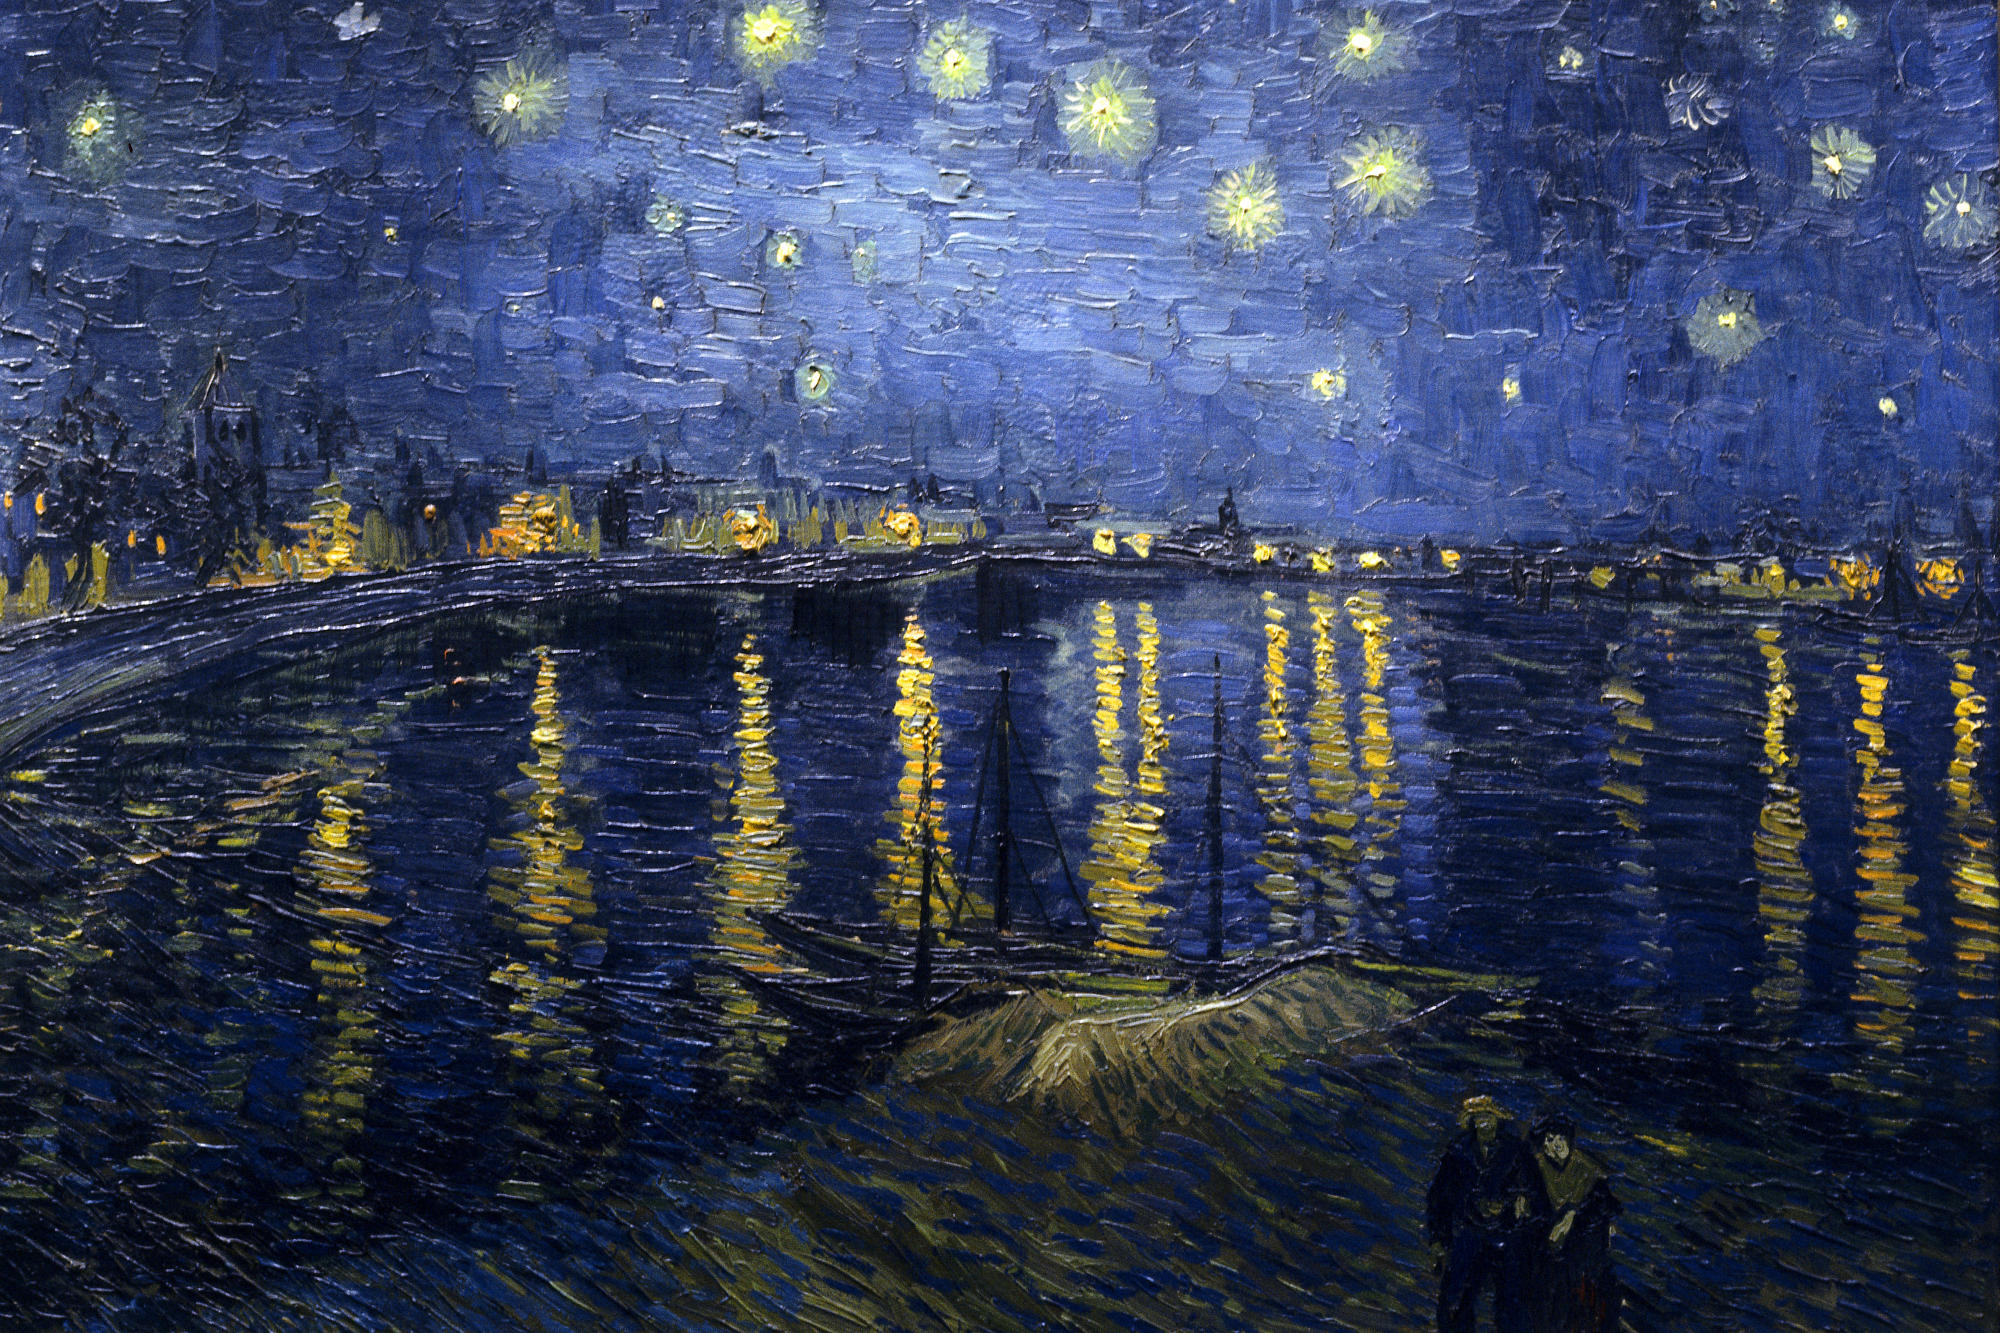
\includegraphics[width=\paperwidth, height=\paperheight]{starryrhone_vangogh_big.jpg}}
%% Questions
\begin{frame}{
	\begin{minipage}[t]{0.75\textwidth}
		Questions
	\end{minipage}
	\hfill
	\begin{minipage}[t]{0.25\textwidth}
		\flushright
		\scalebox{0.035}{
\includegraphics{R_logo.png}}
	\end{minipage}
}{}
%% ==================== Content ===========================%%

\end{frame}

\end{document}